\chapter{Динамические магнитоэлектрические эффекты}\label{ch:ch3}

В данной главе анализируются спектры поглощения и диаграммы фотолюминесценции работ \cite{Toyoda2015, Saito2008prl, Toyoda2016} (см. \cref{sec:ch1/sec3}), а именно - переход на первое возбужденное состояние конфигурации \(3d^9\), отвечающее энергии 1.4 эВ (первый синий пик на \cref{fig:dd_transitions}). Проверяется справедливость гипотезы авторов этих работ о том, что наблюдаемые эффекты можно объяснить в рамках интерференции электрических и магнитных дипольных переходов.

\section{Волновые функции основного и возбужденного состояний}\label{sec:ch3/sect1}

Эффект интерференции матричных элементов электрических и магнитных дипольного переходов крайне чувствителен к виду волновых функций начального и конечного состояний. Таким образом, волновые функции, полученные в \cref{sec:ch2/sec1} для грубой оценки величины поляризации требуют уточнения. Полный гамильтониан системы помимо кристаллического поля содержит операторы спин-орбитального, обменного и зеемановского взаимодействий:

\begin{equation}
	\label{eq:Hamiltonian}
	\hat{H}_{cf}=\sum_{k, q} B_{q}^{k}\hat{C}_{q}^{k}; \; \hat{H}_{so} = \lambda \hat{\bm{l}} \hat{\bm{s}}; \; \hat{H}_{ex}^{g} = J_{gg} \sum_{i=1}^{4} \langle \bm{s}_i \rangle \hat{\bm{s}}; \; \hat{H}_{Z} = \mu_B (\hat{\bm{L}} + 2\hat{\bm{S}}) \bm{B}.
\end{equation}

Параметр спин-орбитального взаимодействия $\lambda \cong -100\,\text{см}^{-1}$. Величина обменного интеграла $J_{gg} \cong 29\,\text{см}^{-1}$ известна по данным о рассеянии нейтронов и по спектрам фотолюминесценции \cite{Toyoda2016, Boehm2002}. 

В рамках бакалаврской выпускной работы нами были получены правила отбора для переходов на компоненты первого возбужденного дублета 1.4 эВ. Расщепление составляло около 5 см$^{-1}$ и было интерпретировано как давыдовское. Впоследствие оказалось, что это не так: в \cite{Kopteva2022} при описании оптических спектров с б\'{о}льшим разрешением выяснили, что расщепление в нулевом магнитном поле на самом деле связано со слабым обменным взаимодействием между возбужденным ионом и окружающими его соседними ионами меди в основном состоянии. Впрочем, в экспериментальных работах \cite{Toyoda2015, Toyoda2016} это обменное поле не проявилось из-за сравнительно большой ширины линий и поэтому ниже не учитывается.

Описание энергетической схемы уровней удобно пояснить методом последовательных приближений. На первом этапе расчета проводится диагонализация оператора \(\hat{H}_{cf}+\hat{H}_{so}\) в базисе всех 10 возможных состояний основной конфигурации $3d^9$ ($^{2}D$). В результате получаются 5 крамерсовских дублетов. На втором этапе, как возмущение, рассчитываются расщепления из-за действия обменного (молекулярного) и внешнего магнитного поля.

Для пояснений картины распределения электронной плотности удобно использовать локальные системы координат с реальным базисом орбитальных волновых функций в дырочном представлении:

\begin{equation}
	\label{eq:BasisFunctions}
	| \epsilon \rangle  = | x^2-y^2 \rangle, \; | \zeta \rangle = | xy \rangle,
	| \theta \rangle  = | 3z^2-r^2 \rangle, \; | \eta \rangle = | xz \rangle, \; | \xi \rangle = | yz \rangle.
\end{equation}

Основным состояниям ионов меди, главным образом, соответствуют состояния типа $| \epsilon \rangle$, а состояниям с энергией $1.4\,эВ$ - $| \zeta \rangle$. При учете спин-орбитального взаимодействия волновые функции основного $| g,\pm \rangle$ и возбужденного $| e,\pm \rangle$ дублетов в локальных системах координат записываются следующим образом:

\begin{equation}
	\label{eq:WaveFunctions}
	\begin{aligned}
		| g,\pm \rangle  = & \; 0.997 \cdot | \epsilon,\pm \rangle \pm 0.069i \cdot | \zeta,\pm \rangle \pm \; 0.025 \cdot | \eta,\mp \rangle - 0.025i \cdot | \xi,\mp \rangle \\
		| e,\pm \rangle = & \; 0.985 \cdot | \zeta,\pm \rangle + 0.112i \cdot | \eta,\mp \rangle	\pm \; 0.112 \cdot | \xi,\mp \rangle \pm 0.062i \cdot | \epsilon,\pm \rangle.
	\end{aligned}
\end{equation}

Отметим, что в работе \cite{Toyoda2015} (см. приложение к работе \cite{Toyoda2015}) примешивание состояний $|\zeta\rangle, \, |\eta\rangle, \, |\xi\rangle$ к волновым функциям основного состояния $|\epsilon\rangle$ не учитывалось. Между тем оно существенно влияет на результаты расчета как расщеплений основного и возбужденного состояния магнитным полем, так и вероятностей электрических дипольных переходов.

Для расчета суммарной интенсивности поглощения требуются волновые функции обеих позиций меди в единой системе координат. Операторы кристаллического поля ${B^\prime}_q^{(k)}$ в кристаллографической системе координат \textit{a}, \textit{b} и \textit{c} связаны с их значениями в локальной системе соотношением:

\begin{equation}
	\label{eq:BkqLocal}
	{B^\prime}_q^{(k)} = B_q^{(k)} exp(-iq\phi).
\end{equation}


\section{Взаимодействие электронов с электромагнитным полем световой волны}\label{sec:ch3/sect2}

Оператор взаимодействия с магнитным полем световой волны записывался в виде:

\begin{equation}
	\label{eq:HM}
	\hat{H}_M = \mu_B (\hat{\bm{L}} + 2\hat{\bm{S}}) \bm{B}^{\omega}.
\end{equation}
При этом учитывалось, что магнитная компонента световой волны связана с электрической соотношением $\bm{B}^\omega \, {=} \, \frac{1}{k} \sqrt{\epsilon\mu} [\bm{k} \times \bm{E}^\omega]$. Согласно экспериментальным данным \cite{Pisarev2011} $\sqrt{\epsilon\mu} \, {\approx} \, 1.75$.

Оператор взаимодействия с электрическим \cref{eq:HE}, как и входящие в него параметры эффективного дипольного момента \cref{eq:Deff} уже были получены нами в параграфе \cref{sec:ch2/sec2}. 

Вместе с тем наши расчеты, показали, что соединение \cbo\ имеет специфическую особенность, затрудняющую точный микроскопический расчет параметров $D_t^{(1k)p}$. При расчете параметров нечетного кристаллического поля вклады от ионов из первой, второй и третьей координационных сфер оказываются примерно одинаковой величины, но разных знаков. В итоге возникает большая погрешность в теоретической оценке величин $D_t^{(1k)p}$. В этой связи возникает необходимость определить минимальных набор подстраиваемых параметров, определяющих электрические дипольные переходы в интересующем нас интервале частот спектра поглощения. Рассчитывая матричные элементы оператора \cref{eq:HE} на волновых функциях \cref{eq:WaveFunctions}, получаем матричные элементы, которые удобно записать следующим образом:

\begin{equation}
	\label{eq:HeMatrixElements}
	\begin{aligned}
		& \langle \epsilon | \hat{H}_E | \eta \rangle = D_1 E_x - D_3 E_y, \\
		& \langle \epsilon | \hat{H}_E | \xi \rangle = D_3 E_x + D_1 E_y, \\
		& \langle \zeta | \hat{H}_E | \eta \rangle = - D_2 E_x - D_4 E_y, \\
		& \langle \zeta | \hat{H}_E | \xi \rangle = D_4 E_x - D_2 E_y.
	\end{aligned}
\end{equation}
Величины $D_i$ связаны с $D_t^{(1k)p}$ соотношениями:

\begin{equation}
	\label{eq:DLabels}
	\begin{aligned}
		& D_1 = \frac{1}{\sqrt{7}} Re \left[ \sqrt{\frac{1}{5}} D_2^{(12)3} + \frac{2}{3} \sqrt{\frac{1}{3}} D_2^{(14)3} + \frac{1}{3} \sqrt{\frac{7}{3 \cdot 5}} D_2^{(14)5} \right], \\
		& D_2 = \frac{1}{\sqrt{7}} Im \left[ \sqrt{\frac{1}{5}} D_2^{(12)3} + \frac{2}{3} \sqrt{\frac{1}{3}} D_2^{(14)3} + \frac{1}{3} \sqrt{\frac{7}{3 \cdot 5}} D_2^{(14)5} \right], \\
		& D_3 = \frac{1}{\sqrt{7}} Im \left[ \sqrt{\frac{1}{5}} D_2^{(12)3} - \frac{1}{2} \sqrt{\frac{1}{3}} D_2^{(14)3} \right], \\
		& D_4 = \frac{1}{\sqrt{7}} Re \left[ \sqrt{\frac{1}{5}} D_2^{(12)3} - \frac{1}{2} \sqrt{\frac{1}{3}} D_2^{(14)3} \right].
	\end{aligned}
\end{equation}

Параметры $D_t^{(1k)p}$, как и параметры кристаллического поля, пропорциональны соответствующим компонентам сферического тензора $C_{-t}^{(p)}$ поэтому при переходе от локальной системы координат в кристаллографическую мы можем использовать соотношение, аналогичное (\ref{eq:BkqLocal}):

\begin{equation}
	\label{eq:DkptLocal}
	{D^\prime}_t^{(1k)p} = D_t^{(1k)p} exp(-it\phi).
\end{equation}
Это соотношение совместно с \cref{eq:BkqLocal} позволяет использовать одинаковые наборы $B_q^{(k)}$ и $D_t^{(1k)p}$ для обеих позиций CuA1 и CuA2.

\section{Сравнение с экспериментальными данными по спектру поглощения}\label{sec:ch3/sect3}

Интенсивность поглощения при переходе с основного $| g \rangle$ на возбужденное состояние $| e \rangle$, вырожденное по спиновым переменным, пропорциональна сумме квадратов модулей матричных элементов по четырем позициям ионов меди в элементарной ячейке.

\begin{equation}
	\label{eq:Ige}
	I_{ge} \sim \sum_\sigma \lvert \langle g | \hat{H}_E + \hat{H}_M | e, \sigma \rangle \rvert^2.
\end{equation}

Из \cref{eq:Ige} видно, что результат сложения матричных элементов операторов $\hat{H}_E$ и $\hat{H}_M$ меняется при обращении направления волнового вектора падающего света. В этой связи можно говорить об интерференции электрических и магнитных дипольных переходов.

На рис. \cref{fig:AbsorptionNonreciprocity}a приведен спектр поглощения из работы\cite{Toyoda2015}. На рис. \cref{fig:AbsorptionNonreciprocity}b приведен результат нашего расчета по формуле (\ref{eq:Ige}).
Параметры электрических дипольных переходов приняты равными (в дебаях):

\begin{equation}
	\label{eq:DParameters}
	D_1 = D_3 = 0.081, \; D_2 = D_4 = 0.085.
\end{equation}

Отметим, что по порядку величины они соответствуют тем, что были получены нами в процессе микроскопического расчета в \cref{sec:ch2/sec2}.

Обратим внимание на то, что по результатам нашего расчета (рис. \cref{fig:AbsorptionNonreciprocity}b) расщепление линий поглощения не симметрично относительно положения линии в нулевом магнитном поле. Имеется линейный по приложенному магнитному полю сдвиг «центра тяжести» в сторону высоких частот. Он обусловлен сдвигом зеемановской компоненты основной состояния вниз по энергии под действием магнитного поля. Этот сдвиг не виден на \cref{fig:AbsorptionNonreciprocity}a. Однако, его прекрасно видно на графиках работы \cite{Kopteva2022}, в которой получены спектры поглощения с б\'{о}льшим разрешением по сравнению с работой \cite{Toyoda2015}. К сожалению, для поляризации света и направления магнитного поля, использованных в \cite{Kopteva2022} явление невзаимности запрещено по симметрии магнитной группы. Как видно из рис. \cref{fig:AbsorptionNonreciprocity} в отношении эффекта невзаимности наши расчеты вполне удовлетворительно соответствуют экспериментальным данным.

\begin{figure}[ht]
	\centerfloat{
		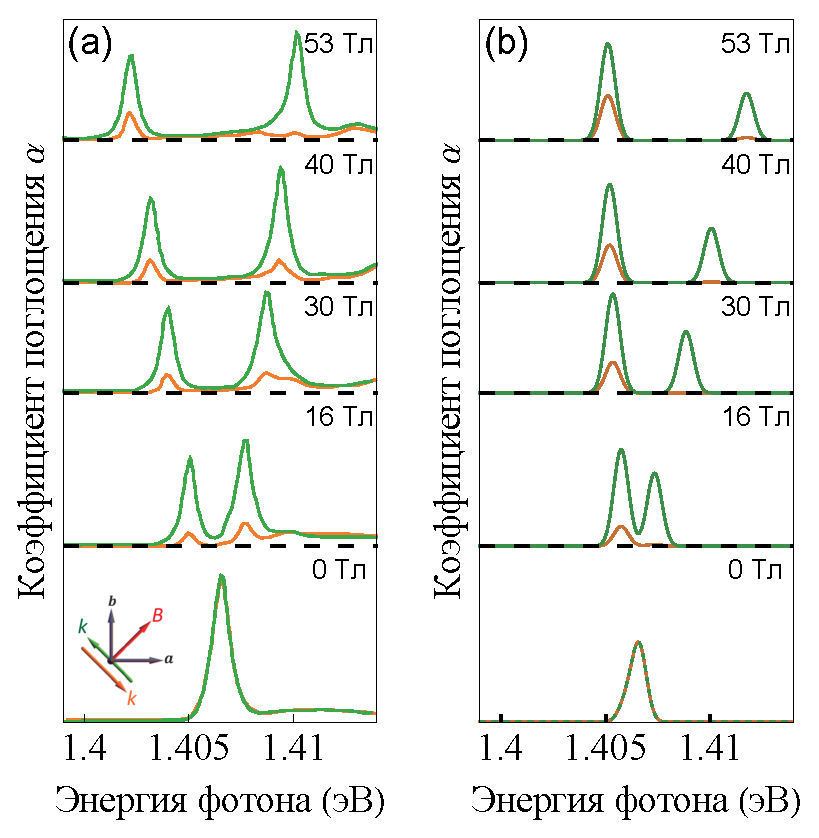
\includegraphics[scale=0.9]{absorption_nonreciprocity}
	}
	\caption{Спектр поглощения света при прохождении через пластинку \cbo. Внешнее магнитное поле $\bm{B} {\parallel} \dir{1}{1}{0}$. Компоненты линейно поляризованной световой волны $\bm{E}^\omega {\parallel} \dir{1}{1}{0}$ и $\bm{H}^\omega {\parallel} \dir{0}{0}{1}$. Зеленым и желтым цветом изображены линии оптического поглощения при направлении волнового вектора света $\bm{k}^\omega {\parallel} \dir{\overline{1}}{1}{0}$ и $\bm{k}^\omega {\parallel} \dir{1}{\overline{1}}{0}$, соответственно. На панели (a) экспериментальные данные из работы \cite{Toyoda2015}, на панели (b) – результаты нашего моделирования без учета неясного происхождения «подставки» в высокочастотной части спектра.}
	\label{fig:AbsorptionNonreciprocity}
\end{figure}

Далее перейдем к анализу результатов экспериментов, проведенных в работе \cite{Saito2008prl}. Из данных приведенных на Рис. 3d видно, что при $\bm{B} {\parallel} \dir{1}{1}{0}$, $\bm{k}^\omega {\parallel} \dir{\overline{1}}{1}{0}$, $\bm{E}^\omega {\parallel} \dir{1}{1}{0}$, $\bm{H}^\omega {\parallel} \dir{0}{0}{\overline{1}}$ эффект невзаимности наблюдается, а при $\bm{B} {\parallel} \bm{k}^\omega {\parallel} \dir{\overline{1}}{1}{0}$, $\bm{E}^\omega {\parallel} \dir{1}{1}{0}$, $\bm{H}^\omega {\parallel} \dir{0}{0}{\overline{1}}$ он отсутствует. Из формулы (\ref{eq:Ige}) следует, что вклад в вероятность перехода, связанный с произведением электрической $E_\alpha^\omega$ и магнитной $H_\beta^\omega$ компонент света, пропорционален компоненте тензора динамической магнитоэлектрической связи:

\begin{equation}
	\label{eq:ChiTensor}
		\chi_{\alpha\beta}^{em} + \chi_{\beta\alpha}^{me} \sim 
		\sim \sum_i \langle g | d_\alpha | e_i \rangle \langle e_i | m_\beta | g \rangle + \langle g | m_\beta | e_i \rangle \langle e_i | d_\alpha | g \rangle,
\end{equation}
где через $d_\alpha$ и $m_\beta$ обозначены эффективные операторы компонент электрического и магнитного дипольных моментов, соответственно. Дипольный момент меняет знак при пространственной инверсии, а магнитный момент – при операции обращения знака времени. Таким образом, динамическая магнитоэлектрическая связь возможна, если одновременно нарушается симметрии и пространственной, и временной инверсии. Кроме того, правая часть (\ref{eq:ChiTensor}) должна быть инвариантна и относительно других операций симметрии (плоскостей отражения, поворотных осей и других) магнитной группы. Магнитная группа определяется пересечением точечной группы симметрии магнитно-упорядоченного кристалла и группы приложенного магнитного поля.

При $\bm{B} {\parallel} \dir{1}{1}{0}$ пересечение кристаллографической точечной группы $D_{2d}$ и магнитной группы дает группу симметрии $m_{x^\prime} m_{y^\prime}^\prime 2_c^\prime$. Здесь и далее, как и в работе \cite{Lovesey2009} оси $x^\prime$ и $y^\prime$ считаются направленными вдоль $\dir{1}{1}{0}$ и $\dir{\overline{1}}{1}{0}$, соответственно. Действуя элементами симметрии $m_{x^\prime}$, $m_{y^\prime}^\prime$ и $2_c^\prime$ на компоненту магнитоэлектрического тензора $\chi_{x^\prime c}^{em} + \chi_{c x^\prime}^{me}$, нетрудно убедиться, что она является инвариантом этой группы, т.е. при $\bm{E}^\omega {\parallel} \dir{1}{1}{0}$, $\bm{H}^\omega {\parallel} \dir{0}{0}{1}$ невзаимность возможна. 

При $\bm{B} {\parallel} \dir{\overline{1}}{1}{0}$ мы имеем магнитную группу симметрии $m_{x^\prime}^\prime m_{y^\prime} 2_c^\prime$. Действуя, например, элементом симметрии $m_{x^\prime}^\prime$ на компоненту $\chi_{x^\prime c}^{em}$ находим, что она изменяет знак, и, следовательно, равна нулю. Таким образом, отсутствие эффекта невзаимности в этом случае легко объясняется.

На Рис. 3c работы \cite{Saito2008prl} приведены результаты экспериментов при $\bm{B} {\parallel} \bm{k}^\omega {\parallel} \dir{0}{1}{0}$, $\bm{E}^\omega {\parallel} \dir{1}{0}{0}$, $\bm{H}^\omega {\parallel} \dir{0}{0}{\overline{1}}$ и при $\bm{B} {\parallel} \bm{k}^\omega {\parallel} \dir{1}{0}{0}$, $\bm{E}^\omega {\parallel} \dir{0}{1}{0}$, $\bm{H}^\omega {\parallel} \dir{0}{0}{1}$. В первом случае невзаимность зарегистрирована, а во втором случае не обнаружена (отсутствует?). Конфигурация направления спинов и поля в первом случае соответствует магнитной группе $2_a 2_b^\prime 2_c^\prime$, а во втором случае – $2_a^\prime 2_b 2_c^\prime$. Действуя элементами симметрии этих групп на компоненту магнитоэлектрического тензора $\chi_{ac}^{em}$ можно установить, что она инвариантна относительно всех операций симметрии группы $2_a 2_b^\prime 2_c^\prime$, но не является инвариантом группы $2_a^\prime 2_b 2_c^\prime$. Таким образом, и в этом случае сценарий интерференции магнитных и электрических дипольных переходов объясняет экспериментальные данные.

Выше были рассмотрены примеры применения микроскопического и теоретико-группового подхода к анализу явления невзаимности в спектре поглощения, которые взаимно дополняют друг друга. Вместе с тем важно отметить, что имеется много вариантов направлений волнового вектора и магнитного поля при которых соображения симметрии оказываются мало эффективными. Сильная сторона микроскопического подхода состоит в том, что он позволяет рассчитывать эффект невзаимности при произвольных направлениях световой волны и внешнего магнитного поля, в том числе и тогда, когда магнитная симметрия достаточно низкая и теоретико-групповой подход оказывается не эффективным. В частности, микроскопический подход позволяет рассчитать эффект невзаимности при отклонении направлений магнитного поля и волнового вектора света от осей симметрии кристалла. Так, допустив небольшие отклонения направления волнового вектора света от оси \textbf{c} кристалла, мы нашли, что «запрещенный» по симметрии эффект невзаимности в геометрии Фарадея $\bm{B} {\parallel} \bm{k}^\omega {\parallel} \dir{0}{0}{1}$  довольно быстро появляется и при отклонениях порядка $3^\circ$ уже вполне может быть зарегистрирован экспериментально. Кстати сказать, это обстоятельство можно использовать для контроля ориентации образцов.

\section{Угловая зависимость интенсивности фотолюминесценции во внешнем магнитном поле}\label{sec:ch3/sect4}

Явление асимметрии в направлении фотолюминесценции (directional asymmetry of luminescence) кристалла \cbo\ обнаружено в работе \cite{Toyoda2016}. Оно зарегистрировано при изменении направления внешнего магнитного поля $\bm{B}$ вдоль \dir{1}{1}{0} на противоположное. Компоненты волны поляризованы следующим образом: $\bm{E}^\omega {\parallel} \dir{1}{1}{0}$, $\bm{H}^\omega {\parallel} \dir{0}{0}{1}$. Согласно общей теории излучения, естественно считать, что предпочтительным направлением люминесценции является такое, при котором вероятность перехода между исходным и конечным состояниями имеет наибольшее значение. В этом плане явления асимметрии люминесценции и невзаимность в спектре поглощения – это два разных оптических явления, имеющих общее происхождение. Однако для практических приложений наибольший интерес представляют диаграммы излучения для различных произвольных направлений волнового вектора. Результаты наших расчетов приведены на рис. \cref{fig:LuminescenceEab, fig:LuminescenceEyc, fig:LuminescenceHyc}.

\begin{figure}[ht]
	\centerfloat{
		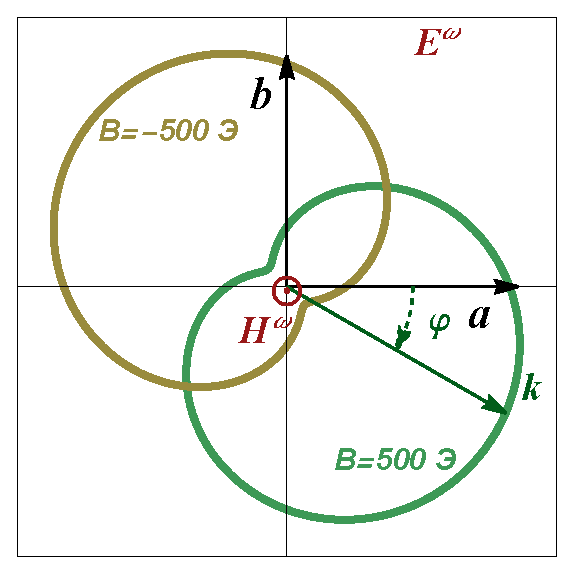
\includegraphics[scale=0.7]{luminescence_Eab}
	}
	\caption{Рассчитанная диаграмма относительной интенсивности фотолюминесценции в плоскости \textit{ab} монокристалла \cbo\ при переключении направления внешнего магнитного поля $B {=} \pm500 \, Э$ вдоль направления $\dir{1}{1}{0}$. Длина полярного вектора (вдоль волнового вектора излучения $\bm{k}^\omega$) считается пропорциональной вероятности суммарного электрического и дипольного переходов из возбужденных состояний $| e, \pm \rangle$ в основное $| g, - \rangle$, т.е. сумме $\sum_\sigma \lvert \langle g | \hat{H}_E + \hat{H}_M | e, \sigma \rangle \rvert^2$. Предполагается, что вектор антиферромагнетизма $\bm{L} {\parallel} \dir{1}{\overline{1}}{0}$. Компонента световой волны $\bm{H}^\omega$ осциллирует вдоль оси \textbf{c}.}
	\label{fig:LuminescenceEab}
\end{figure}

\begin{figure}[ht]
	\centerfloat{
		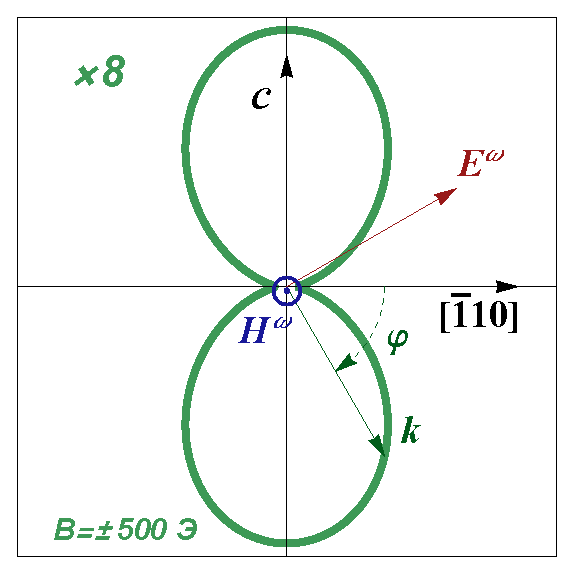
\includegraphics[scale=0.7]{luminescence_Eyc}
	}
	\caption{Рассчитанная диаграмма изменения относительной интенсивности фотолюминесценции для однодоменного образца при изменении направления внешнего магнитного поля $B {=} \pm500 \, Э$, перпендикулярно плоскости рисунка. $\bm{L} {\parallel} \dir{1}{\overline{1}}{0}$, $\bm{H}^\omega {\parallel} \dir{1}{1}{0}$, $\phi$ отсчитывается от направления $\dir{\overline{1}}{1}{0}$. Максимальное значение интенсивности примерно в 8 раз меньше её значения на рис. \cref{fig:LuminescenceEab}.}
	\label{fig:LuminescenceEyc}
\end{figure}

\begin{figure}[ht]
	\centerfloat{
		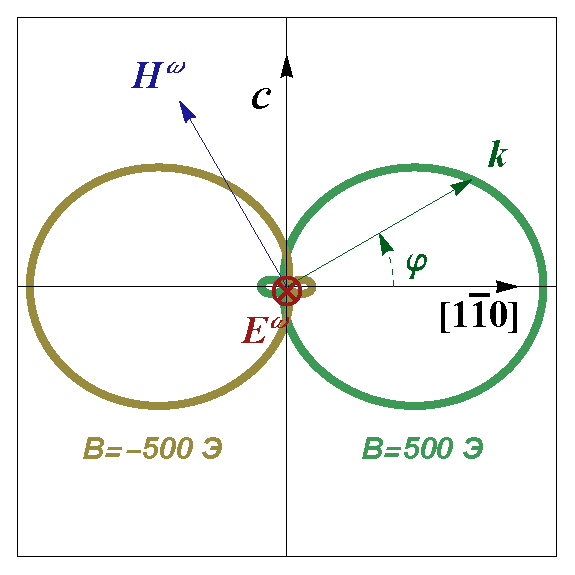
\includegraphics[scale=0.7]{luminescence_Byc}
	}
	\caption{Рассчитанная диаграмма изменения относительной интенсивности фотолюминесценции для однодоменного образца при изменении направления внешнего магнитного поля $B {=} \pm500 \, Э$, перпендикулярно плоскости рисунка. $\bm{L} {\parallel} \dir{1}{\overline{1}}{0}$, $\bm{E}^\omega {\parallel} \dir{1}{1}{0}$, $\phi$ отсчитывается от направления $\dir{1}{\overline{1}}{0}$.}
	\label{fig:LuminescenceHyc}
\end{figure}

Отметим, что диаграмма асимметрии фотолюминесценции на рис. \cref{fig:LuminescenceEyc} ($\bm{B} {\parallel} \dir{1}{1}{0}$, вектор антиферромагнетизмa $\bm{L} {=} \bm{S}_{A1} {-} \bm{S}_{A2} {\parallel} \dir{1}{\overline{1}}{0}$, $\bm{E}^\omega {\parallel} \dir{1}{1}{0}$, $\bm{H}^\omega {\parallel} \dir{0}{0}{1}$) соответствует экспериментальным данным на рис. \cref{fig:ndd}b. Тот факт, что асимметрия люминесценции в геометрии Фарадея, т.е. $\bm{B} {\parallel} \bm{k}^\omega {\parallel} \dir{1}{1}{0}$, отсутствует, можно легко понять на основе соображений симметрии, как это пояснялось при описании невзаимности в спектрах поглощения.

\clearpage
